\section{Problem Formulation}
\label{sec:problemformulation}

% Organization of the Sec
In this section, we describe the multi-band multi-radio wireless mesh network architecture, and formulate the key research issue channel assignment. 
We propose a linear program to understand the architecture and illustrate the challenges of the problem.
Then we leverage the factors of the performance for multi-band wireless network.
 
\subsection{Multiband Wireless Mesh Network Architecture}
\label{subsec:architecture}
~\emph{Wireless Mesh Network} could be chopped as two-tiers:
Access layer, consists of static traffic aggregation mesh nodes for clients, and backhual layer for interconnection from mesh nodes to gateway nodes with wired Internet connection ~\cite{akyildiz2005wireless}. 
~\emph{Multiband Wireless Mesh Network} is for backhual layer, since access layer always need ISM band channels providing access to client's Wifi devices, such as iPhone, laptops. To simply the analysis, we assume the backhual layer uses different channels in ISM band from access layer.

% Explain multiband vs multichannel
A lot of efforts have been put on the similar architecture ~\emph{Multichannel Multi-radio Mesh Network} focusing on ~\emph{Channel Assignment, Multihop Routing, Gateway Placement} problems ~\cite{si2010overview}.
In these works, ~\emph{Multichannel} is a word mention multiple frequency channels have the same propagation performance with small frequency gap, for instance the orthogonal WLAN channels in 2.4GHz from 2.412GHz to 2.484GHz with 22MHz gap.
We refer ~\emph{Multiband} as a combination of different frequency of large gap whose propagation characteristics are different, such as a combination one channel in 2.4GHz and one channel in 900MHz.

%A node in ~\emph{Multiband Wireless Mesh Network} has limited multiple slots for installing radios working in different bands. 
%Two nodes share the same link should have a common channel. The sum of the loads on the links should 
% Explain propagation, factors of the environment and so on
Wireless propagation is the behavior of the signal loss characteristics when they are transmitting from one point to another.
The factors rule radio propagation are complex and diverse, 
such as the daily changes of environment, weather, and atmosphere changes due to cosmos activities. 
In most propagation models there are three basic propagation mechanisms: reflection, diffraction, and scattering ~\cite{andersen1995propagation}.
For multiband mesh backhual network, the nodes are usually installed on the top of buildings or towers. That makes a line of sight propagation model is a reasonable hypotheses for multiband mesh.
% propagation fomular, explain the band influence
In \emph{Friis} propagation model, the received signal power of a node is represented as: 
\begin{equation}
\label{eq:friis}
P_r=P_t+G_t+G_r+20log_{10}(\frac{\lambda}{4\pi R})
\end{equation}

Path-loss exponent \emph{$\alpha$} is used to describe the environment factors, typically in outdoor environments range from 2 to 5.\cite{camp2006measurement}. 
In ~\ref{eq:friis}, the received signal could vary only due to the wavelength $\lambda$ represents band. 
This variation makes the performance of radios in multiple bands different even under the same configuration in the same location. Since the radios have the same received signal threshold, lower frequency band could have a larger communication range $R$, and also a larger interference range $I_r$.

%In multiband scenario, both wired ~\emph{Gateway Nodes} and ~\emph{Mesh Nodes} are equipped with multiple radios working in different frequency band, including ISM bands and white space bands. The radios could work simultaneously bringing more capacity to the network which is a evolution of ~\emph{Multi-channel Multi-Radio Mesh Network} with radios working in the same band in different channels.

\begin{figure}                                                                                                                     
%\vspace{-0.0in}
\centering
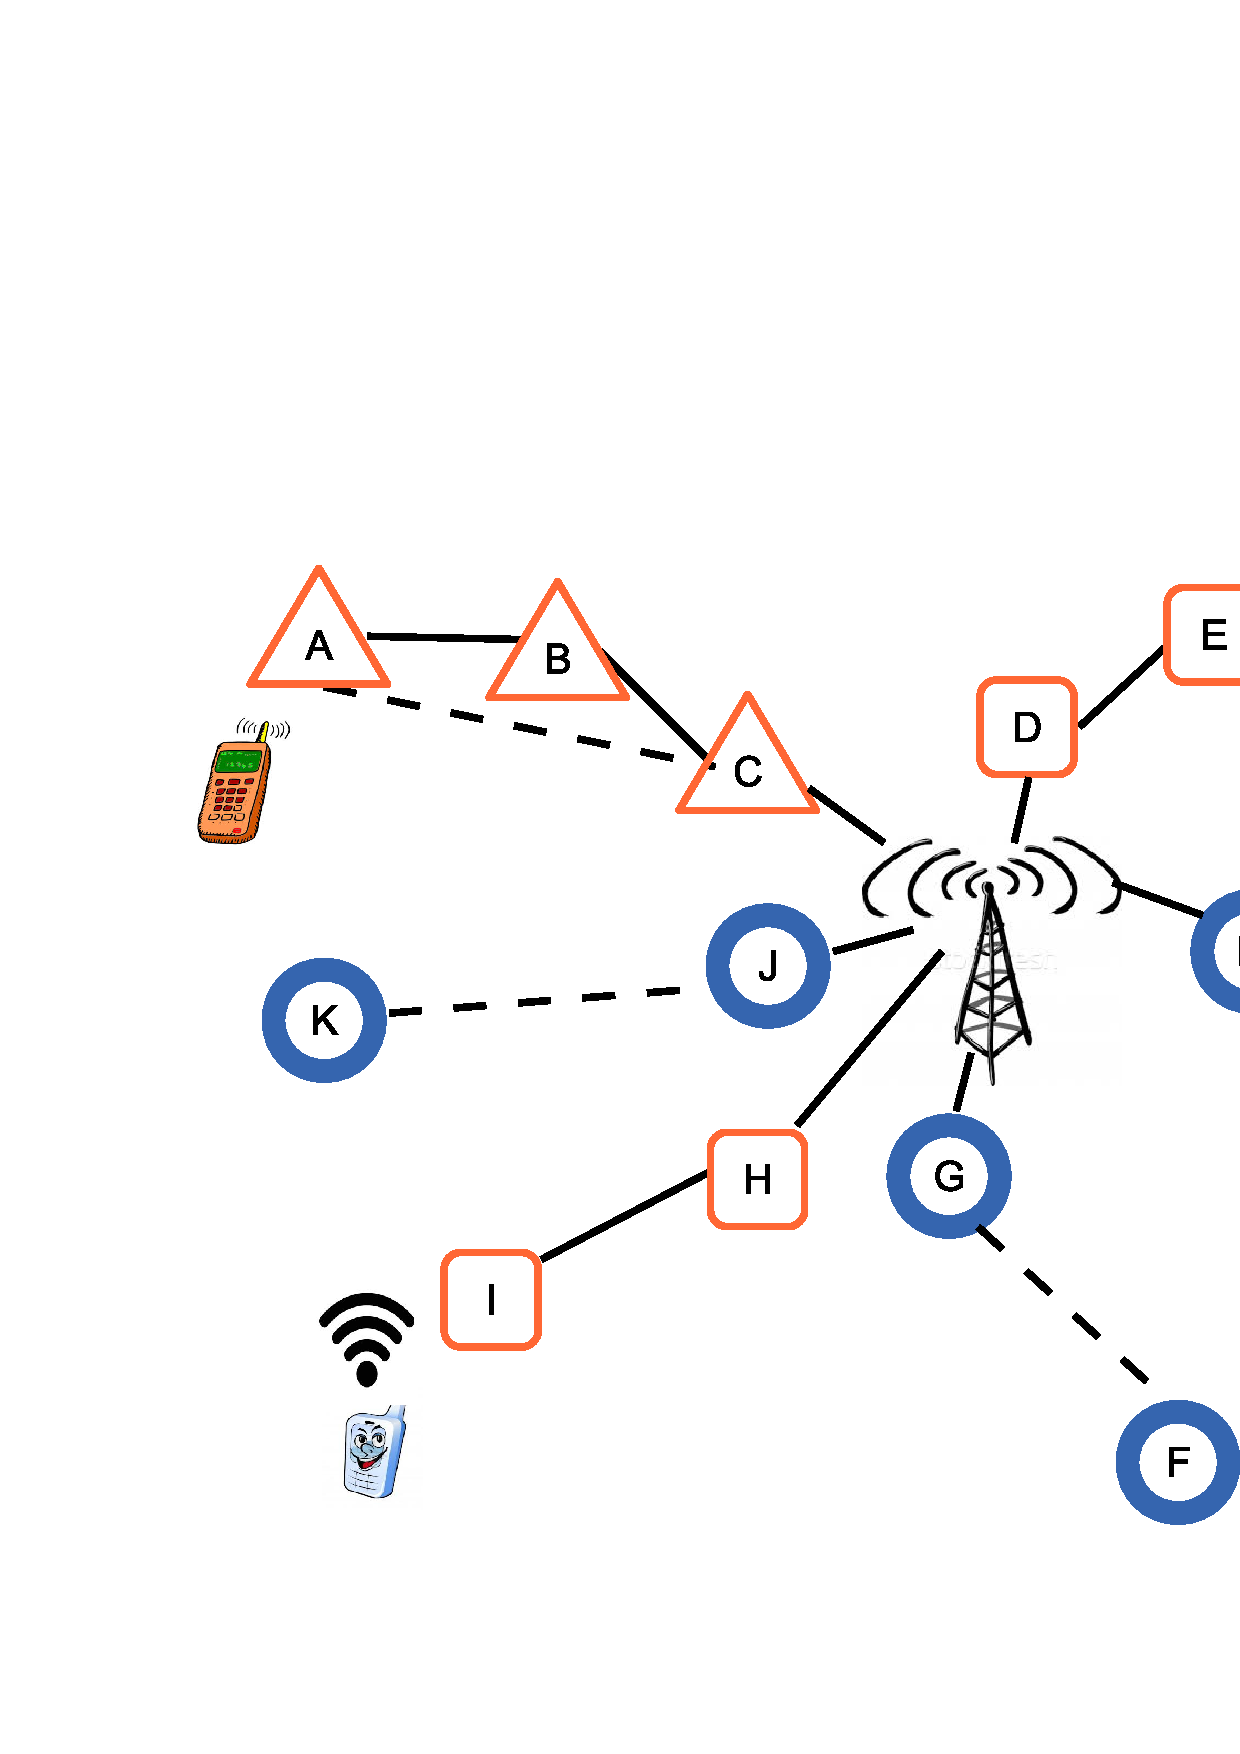
\includegraphics[width=74mm]{figures/interferencerange}
\vspace{-0.1in}
\caption{Multiband Communication and Interference Range}
\label{fig:interferencerange}
%\vspace{-0.0in}
\end{figure}


% Make multiband challenges
The broadcast nature of the wireless medium makes it generate multiple access interference in wireless network.
Employing ~\emph{White Space Band} in lower frequency brings advantages for mesh network, 1) more orthogonal bandwidth reduce the contention and conflict in the network,
 2) the propagation variation brings flexible topology by reducing connection hop counts in the network.
However, at the same time, links in ~\emph{White Space Band} also increase the interference range in the network making space reuse of the white space band channel difficult. 
In \ref{fig:interferencerange}, node ~\emph{N1} could connect to node ~\emph{N3} through relay of node ~\emph{N2} in higher frequency band, or directly connect by lower frequency band channel with larger communication range.
If under higher frequency band, link between node ~\emph{N4} and node ~\emph{N5} could reuse the higher frequency since they are out of the interference range of this high frequency band; 
however, if \emph{N1} and ~\emph{N3} connected with lower frequency band in less hop counts, then ~\emph{N4} and ~\emph{N5} could not reuse these lower frequency channels due to the larger interference range.
To balance the larger communication range and larger interference range of white space band is a key issue in ~\emph{Multiband Mesh Network Channel Assignment} different from ~\emph{Multichannel} scenario.

\subsection{Model and Problem Formulation}
\label{subsec:problem}

% Assumptions of the network
~\emph{Channel Assignment} is to assign radios between nodes in mesh network creating virtual links for network communication with minimum interference.
Our objective is to get a channel assignment for a wireless mesh network formed by a set of static mesh nodes and wired gateway nodes. 
Each node in the network is equipped with one or more radios could work in one of the permitted bands. 
%FIXME keep or not
%To clarify the ~\emph{White Space Band} influence, we assume radios in a node works in unique non-overlapping channels of multiple band, radios in two nodes share a common channel in the same band.
We also assume all the nodes have the same configuration, each radio works under the same transmitting power, antenna with the same gains.
To model the connectivity, we adopt classical ~\emph{Protocol Model} from Gupta ~\cite{gupta2000capacity}. If the received signal is above the threshold, the link would have a communication capacity, otherwise, the link could not exist.
In ~\emph{Protocol Model}, the interference exist as conflict contention when the received signal strength of other links are above the threshold; otherwise, the link will not be interfered by other links.

The ~\emph{Gateway Nodes} and ~\emph{Mesh Nodes} locations are given. 
%In a network, ~\emph{Channel Assignment} naturally binds with a routing protocol for application, but have different target. We bind our model with a ~\emph{Shortest Path Routing} protocol for ~\emph{Channel Assignment} application and evaluation.
Other input information includes, transmitting power, antenna gains, communication and interference threshold. From ~\emph{Friis Model}, we could get ~\emph{Communication Range} and ~\emph{Interference Range} of each link in different band. 
Multiband multi-radio wireless network could be formulated as an undirected graph $G=(V,E)$ according to the communication range and interference range. $V$ is noted as the nodes, and $E$ marked as the links in the network.

The channel assignment is represented as ~\emph{Connectivity Graph}, $C=(V,L,B)$, $L$ denotes the set of links, $B$ denotes the set of frequency bands. 
The capacity between two nodes in common channel is noted as $C_{lb}, l \in L,b \in B$. If they are physically located within each others communication range of a band, the value of $C_{lb}$ would be a constant value, otherwise, it is zero. 

The associated interference range is larger than the communication range for each node. We extend the ~\emph{Conflict Matrix} from Jain's work with a flexible approach for interference, $CG=(L_{i,j},I_{Set},B)$. $L_{i,j}$ represents the active link, $I_{Set}$ includes all the links are physically inside the interference range. 

Our model is similar to ~\emph{Multichannel Model} in many previous works ~\cite{tang2005interference,yuan2006cross,si2010overview}. However, in ~\emph{Multichannel Model}, the ~\emph{Communication Range} and ~\emph{Interference Range} in different channels are the same. The ~\emph{Multichannel Model} is unnecessary to consider the variation of range due to band propagation.
~\emph{Multiband Channel Assignment} work toward the same target as ~\emph{Multichannel Channel Assignment} to provide richer connectivity with minimum interference.

The difficulty of the problem is that we can not know the interference before we assign channel to each node. Previous works have proposed ~\emph{Coloring, Cluster, Independent Set, Mixed Linear Integer} methodology to approach the solution of ~\emph{Multichannel Channel Assignment} ~\cite{mishra2005weighted,peng2012efficient,tang2005interference}. 
However, these work fails to distinguish the trading off between minimize hops and more frequency space reuse among multiple bands.
Our work focus on the ~\emph{traffic-independent} 
without explicitly considering network traffic/load ~\cite{marina2010topology}.
To approach the optimization channel assignment, we develop a mixed linear integer model to understand the multiband scenario. We also analyze the intra-relation between the ~\emph{Hop Counts} and ~\emph{Space Reuse}, then propose two heuristic approaching for this problem.

\subsection{Evaluation Metric}
\label{subsec:metric}
~\emph{Mesh Network} is designed to provide service for clients. The goal of a backhual network is to maximize its overall good put within a unit time. 
This enables the network to support more end-user flows, and in turn more number of users. To evaluate the assignment, we use the idea of ~\emph{Gateway Good put} of the network. The gateway good put X of a network is defined as

\begin{equation}
\label{eq:goodput}
X=\sum_{g \in G, v \in V}C(g,v)
\end{equation}

In ~\cite{robinson2008adding}, Robinson proves the bottle neck of mesh network capacity is the gateway wireless connection. 
The gateway good put is the traffic arrive at the gateway node and relay to the wired Internet. The good put performance is correlated with gateway placement, channel assignment and routing. 
The calculation of ~\emph{Gateway Good put} is described in ~\ref{sec:experiment design} .Jointly optimization of channel assignment, gateway placement, and routing is out of the scope of this paper.

